\documentclass[12pt]{article}

\usepackage[margin=1in]{geometry}
\usepackage[version=3]{mhchem}
\usepackage{graphicx}
\usepackage{subfig}
\usepackage{fancyhdr}
\usepackage{amsmath}

\newcommand{\unit}[1]{\ensuremath{\, \mathrm{#1}}}
\newcommand{\e}[1]{\ensuremath{\times 10^{#1}}}

\pagestyle{fancy}
\lhead{NANO 266 - Quantum Mechanical Modeling}
\rhead{Spring 2015}

\title{NANO 266 - Lab 2}
\author{Zhi Deng \\ PID:A53058446}
\date{Apr 20, 2015}

\begin{document}

\maketitle
\thispagestyle{fancy}

\section*{Q1}

\begin{figure}[h]
\begin{center}
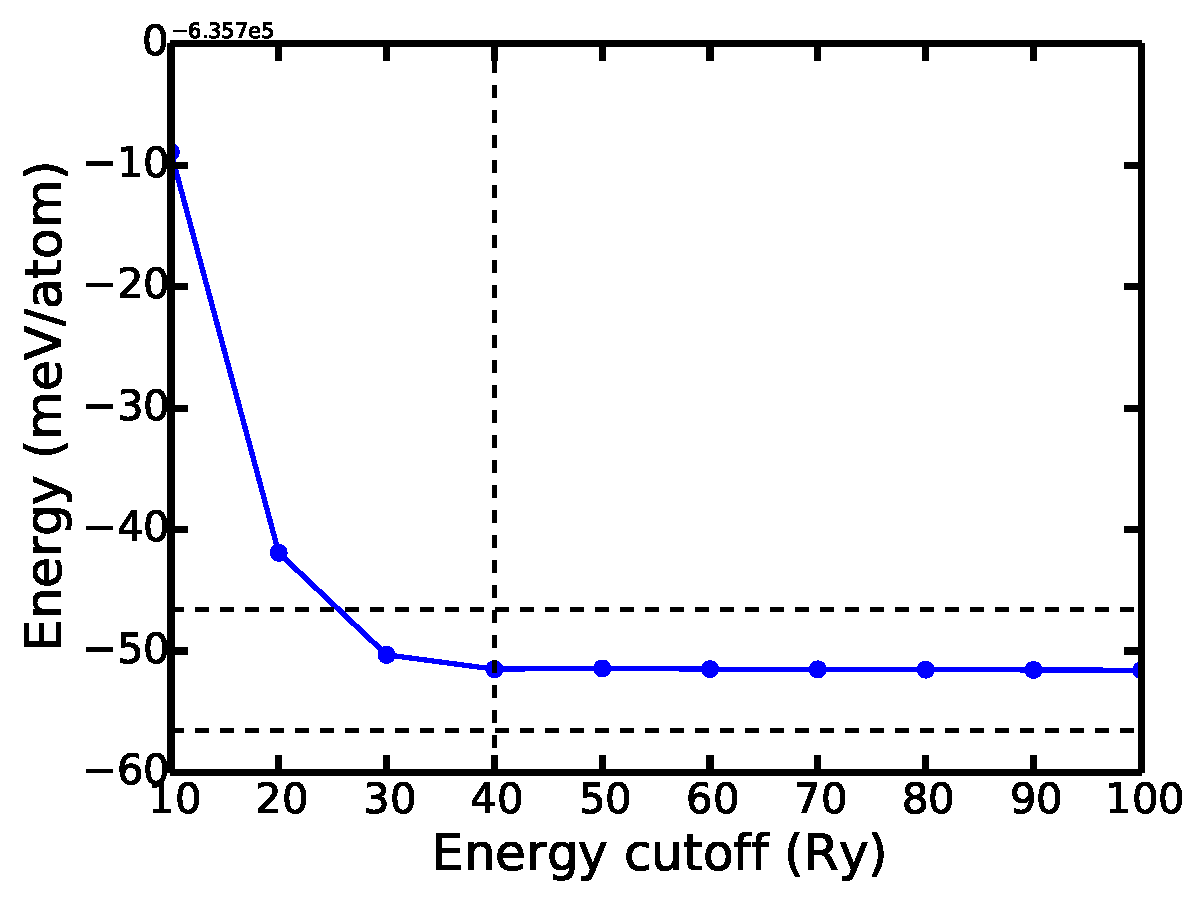
\includegraphics[width=.5\textwidth]{Q1}
\end{center}
\end{figure}

The absolute energy is reaching a converged value as the energy cutoff increases. Convergence occurs after the energy cutoff reaching 40 \unit{Ry}. 

\clearpage

\section*{Q2}

\begin{figure}[h]
\begin{center}
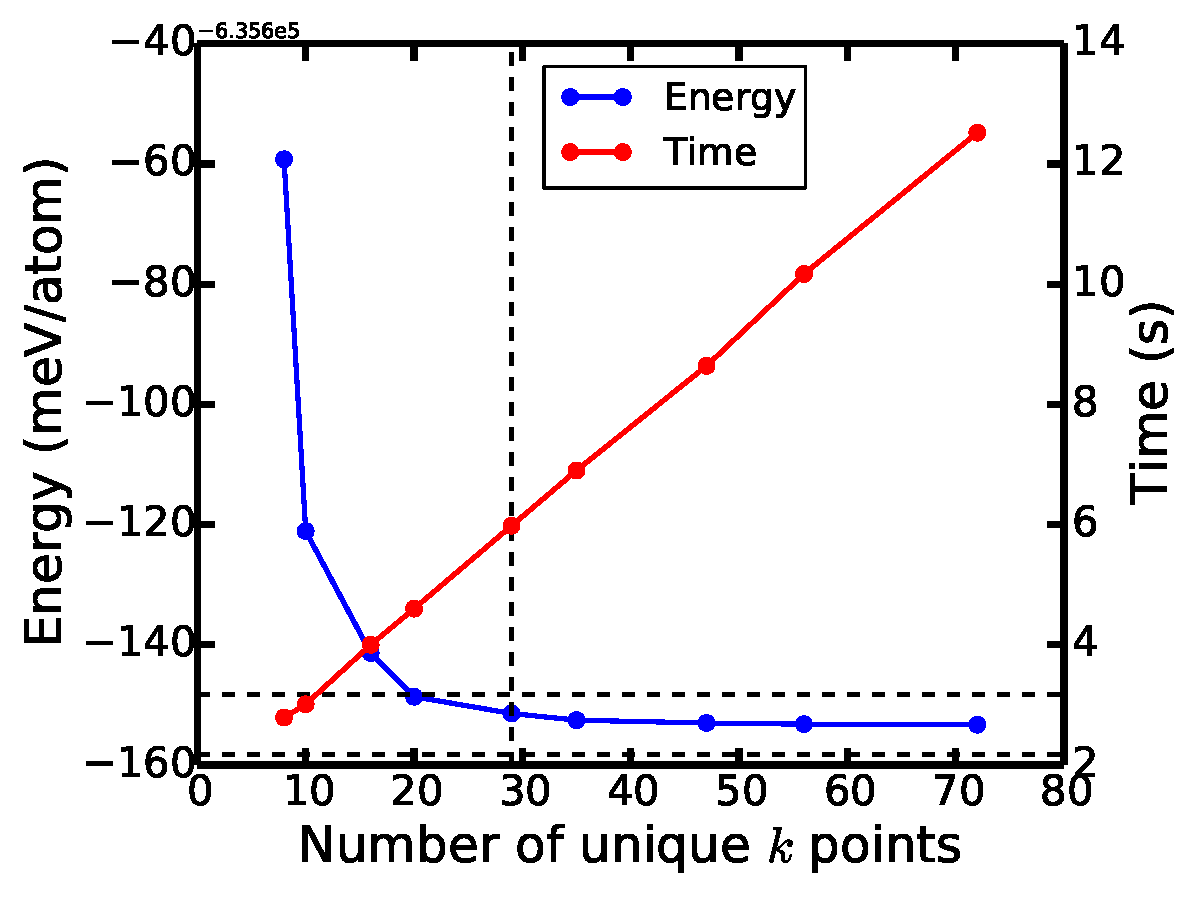
\includegraphics[width=.5\textwidth]{Q2}
\end{center}
\end{figure}

The absolute energy is reaching a converged value as the density of $k$-point grid increases. Convergence occurs after $k$-point grid size reaching $8\times8\times8$. 

The CPU time used linearly increases with the number of unique $k$ points. 

\section*{Q3}

Lattice parameter: $a = 10.26\unit{a.u.}$

\noindent Atomic positions: $\begin{pmatrix}0 & 0 & 0.05\end{pmatrix}$, $\begin{pmatrix}0.25 & 0.25 & 0.25\end{pmatrix}$

\noindent $k$-point grid: $4\times4\times4$

\begin{figure}[h]
\begin{center}
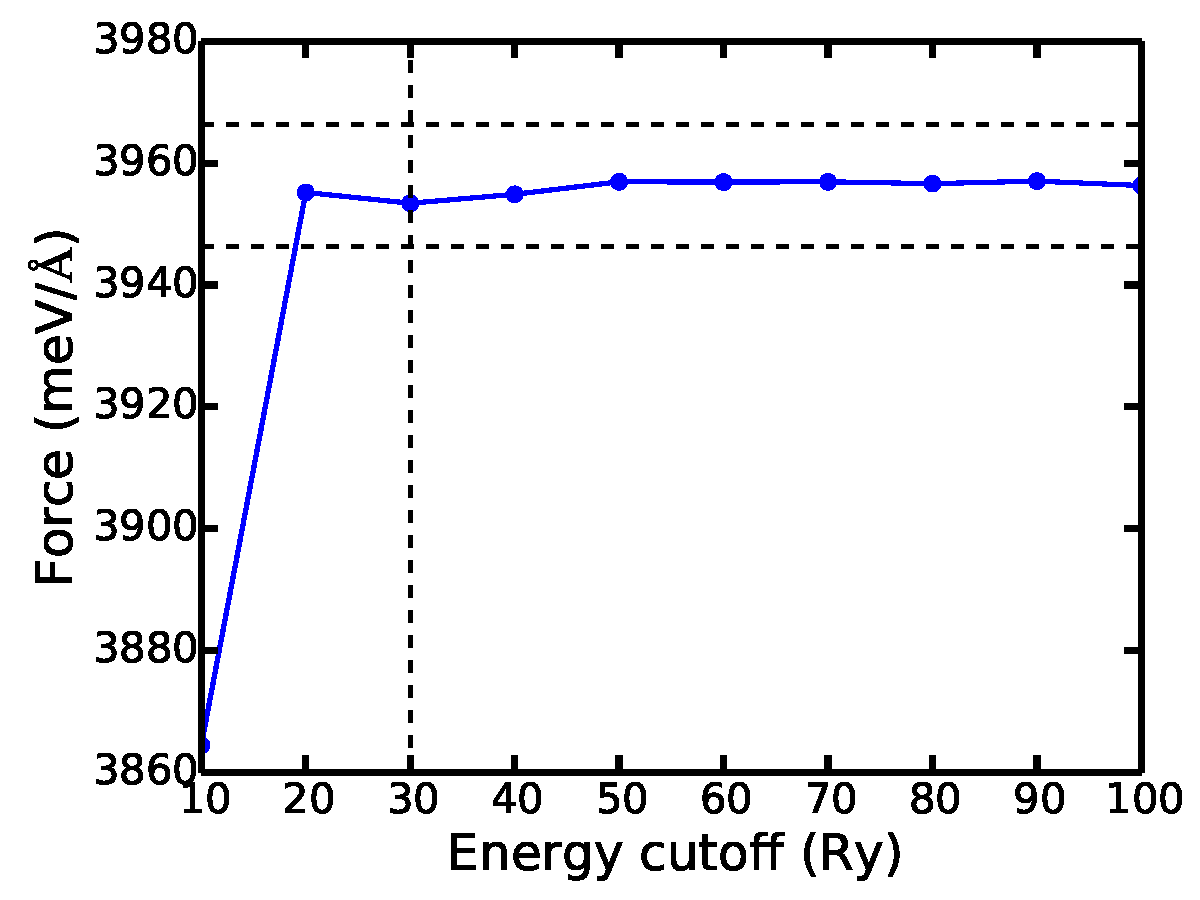
\includegraphics[width=.5\textwidth]{Q3}
\end{center}
\end{figure}

The total force is reaching a converged value as the energy cutoff increases. Convergence occurs after the energy cutoff reaching 30\unit{Ry}. 

\section*{Q4}

Lattice parameter: $a = 10.26\unit{a.u.}$

\noindent Atomic positions: $\begin{pmatrix}0 & 0 & 0.05\end{pmatrix}$, $\begin{pmatrix}0.25 & 0.25 & 0.25\end{pmatrix}$

\noindent Energy cutoff: 30 \unit{Ry}

\begin{figure}[h]
\begin{center}
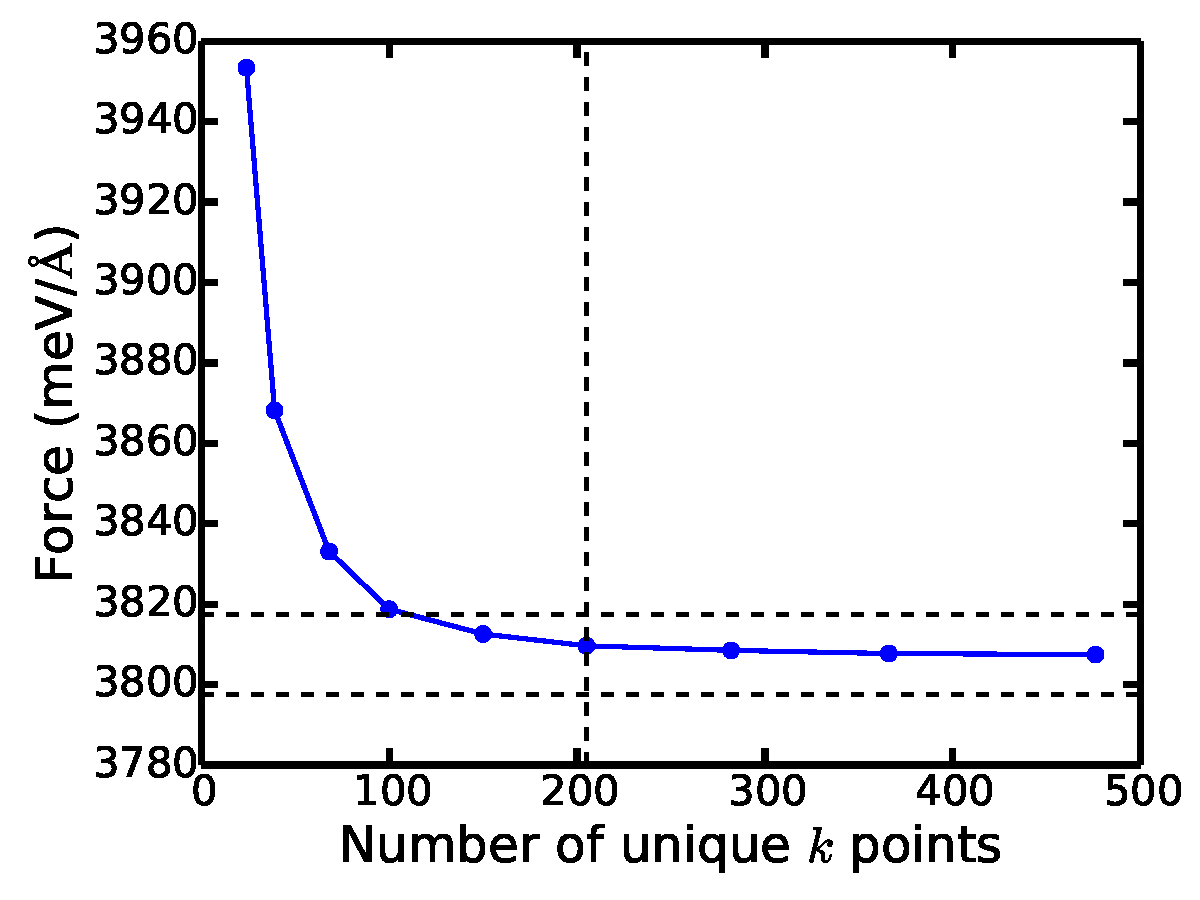
\includegraphics[width=.5\textwidth]{Q4}
\end{center}
\end{figure}

The total force is reaching a converged value as the density of $k$-point grid increases. Convergence occurs after $k$-point grid size reaching $9\times9\times9$. 

\section*{Q5}

2 set of lattice parameters: $a = 10.26\unit{a.u.}$, $a = 10.30\unit{a.u.}$

\begin{figure}[h]
\begin{center}
\subfloat[Fixed $k$-point grid $8\times8\times8$]{
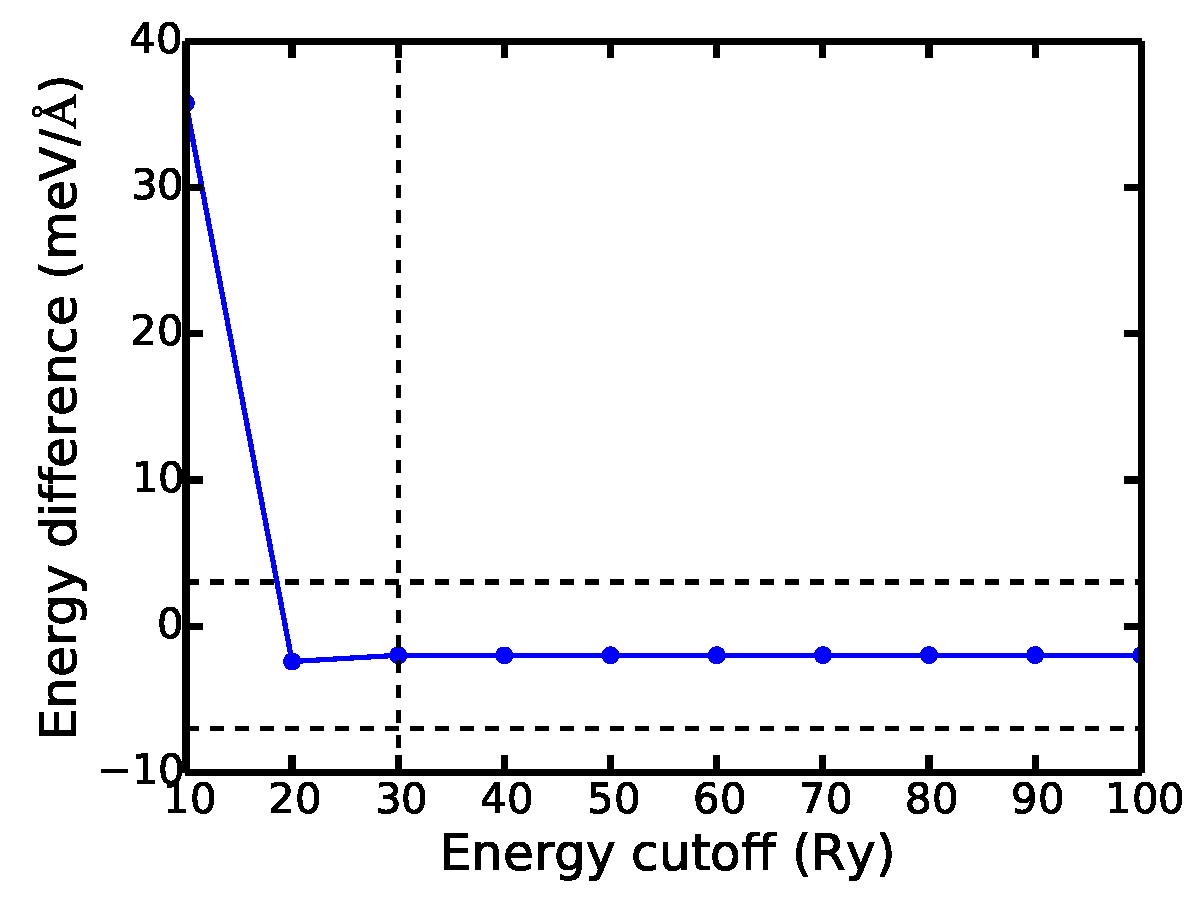
\includegraphics[width=.45\textwidth]{Q5_e}
}
\subfloat[Fixed energy cutoff 30\unit{Ry}]{
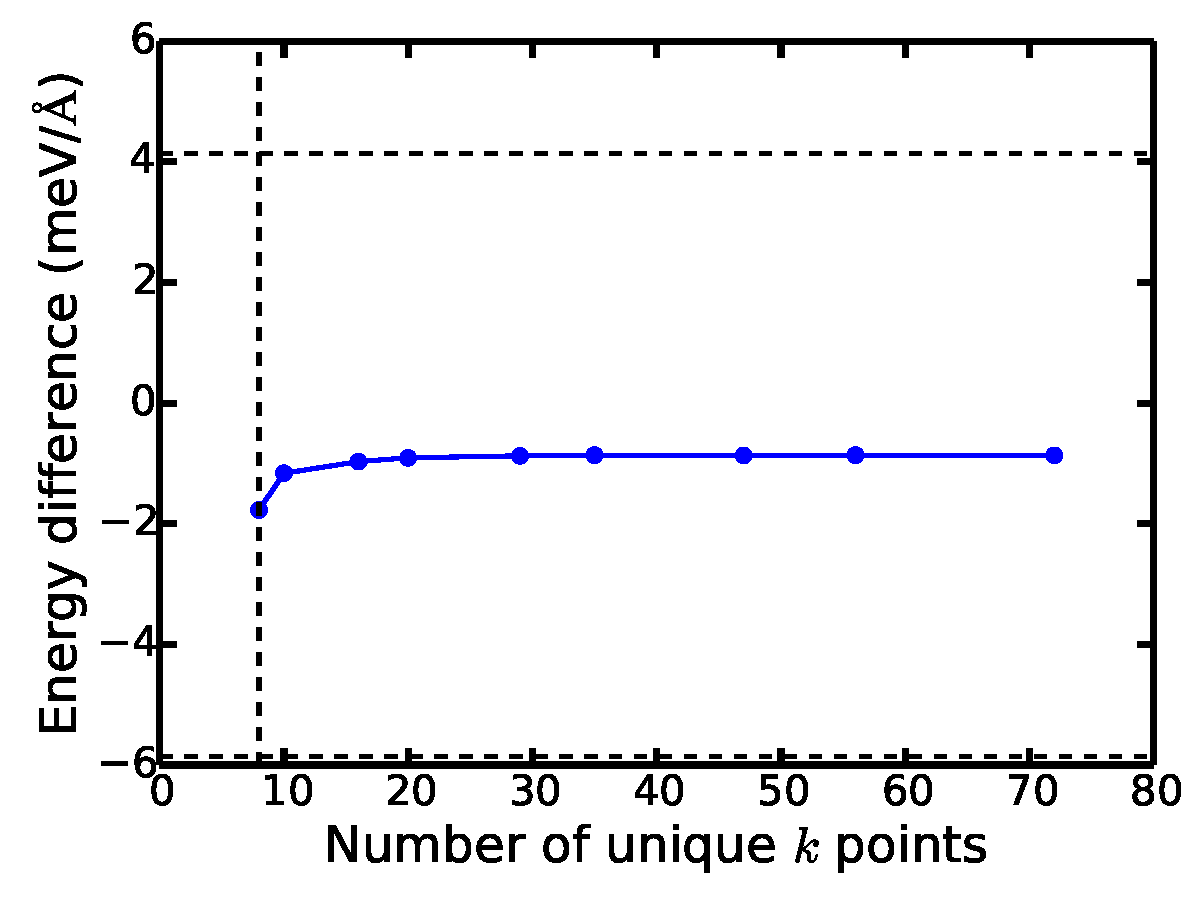
\includegraphics[width=.45\textwidth]{Q5_k}
}
\end{center}
\end{figure}

The energy difference is reaching a converged value as the energy cutoff or the density of $k$-point grid increases. Convergence occurs after the energy cutoff reaching 30\unit{Ry}, or the $k$-point grid size reaching $4\times4\times4$.

\section*{Q6}

All calculated properties (absolute energy, total force and energy difference) reach convergence at certain high energy cutoff and certain high density $k$-point grid. Higher energy cutoff allows wavefunctions with higher energy, thus increasing the overall accuracy. Higher density $k$-point grid means that the integrations are done with more points in the same space, leading to higher accuracy as well. The convergence of absolute energy has a higher criteria in both energy cutoff and $k$-point grid. For total force, the criteria slightly loose in energy cutoff. While for energy difference, the convergence has the lowest criteria. We need to choose the right parameters based on the property of interests. 

\section*{Q7,8}

To ensure the convergence of absolute energy, an energy cutoff of 40\unit{Ry} and a $8\times8\times8$ $k$-point grid were applied. Perform static calculations near the lattice constant at equilibrium. Plot the total energy (per cubic cell) as a function of lattice constant. 

\begin{figure}[h]
\begin{center}
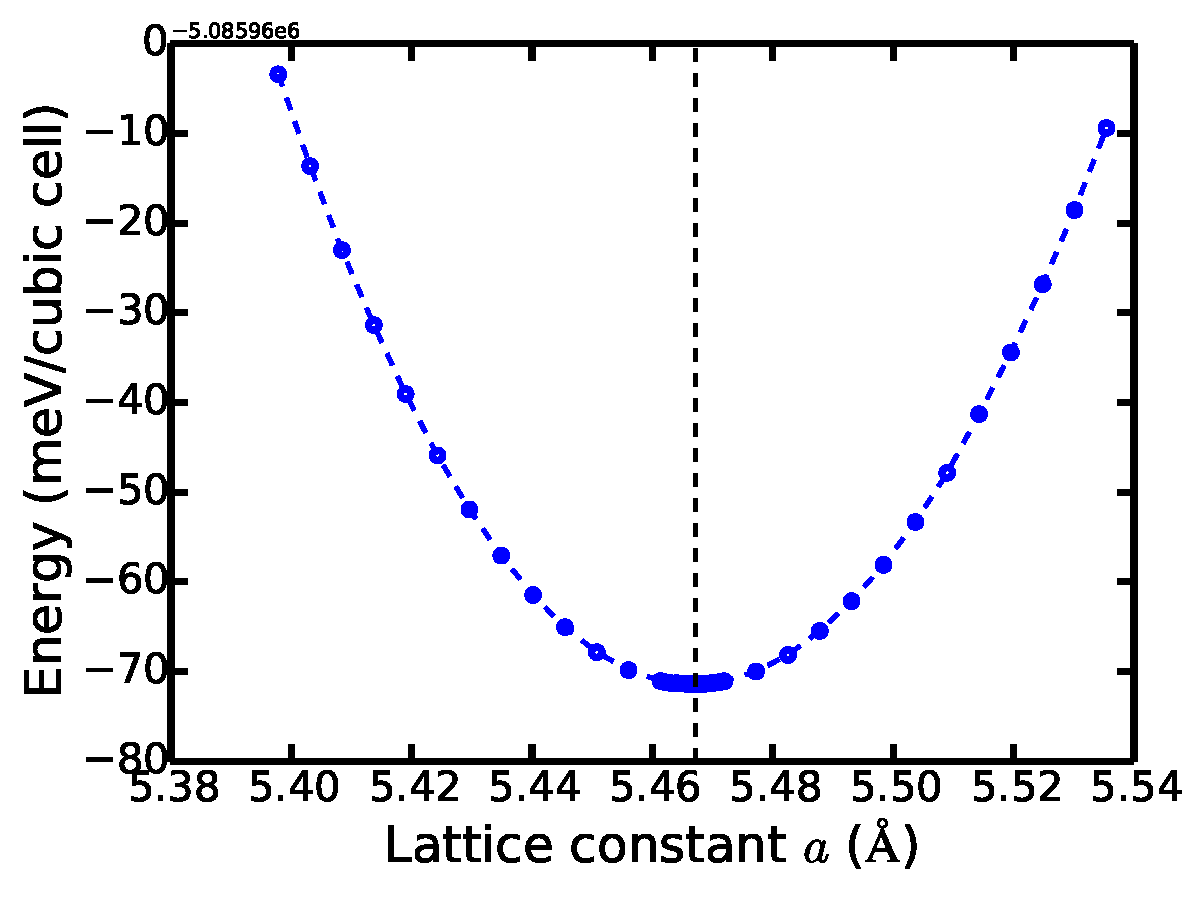
\includegraphics[width=.6\textwidth]{gga_a}
\end{center}
\end{figure}

The lattice constant of equilibrium structure is $a_0 = 10.331\unit{a.u.} = 5.4672\unit{\AA}$. 

The bulk modulus is given by:
\begin{flalign*}
K = V_0\left.\frac{\partial^2 E}{\partial V^2}\right|_{V = V_0}
\end{flalign*}
To calculate the bulk modulus, first plot the total energy as a function of volume. This is achieved by converting the lattice constant to the volume of the cubic cell ($V = a^3$) on the $E$-$a$ plot. 

\clearpage
\begin{figure}[h]
\begin{center}
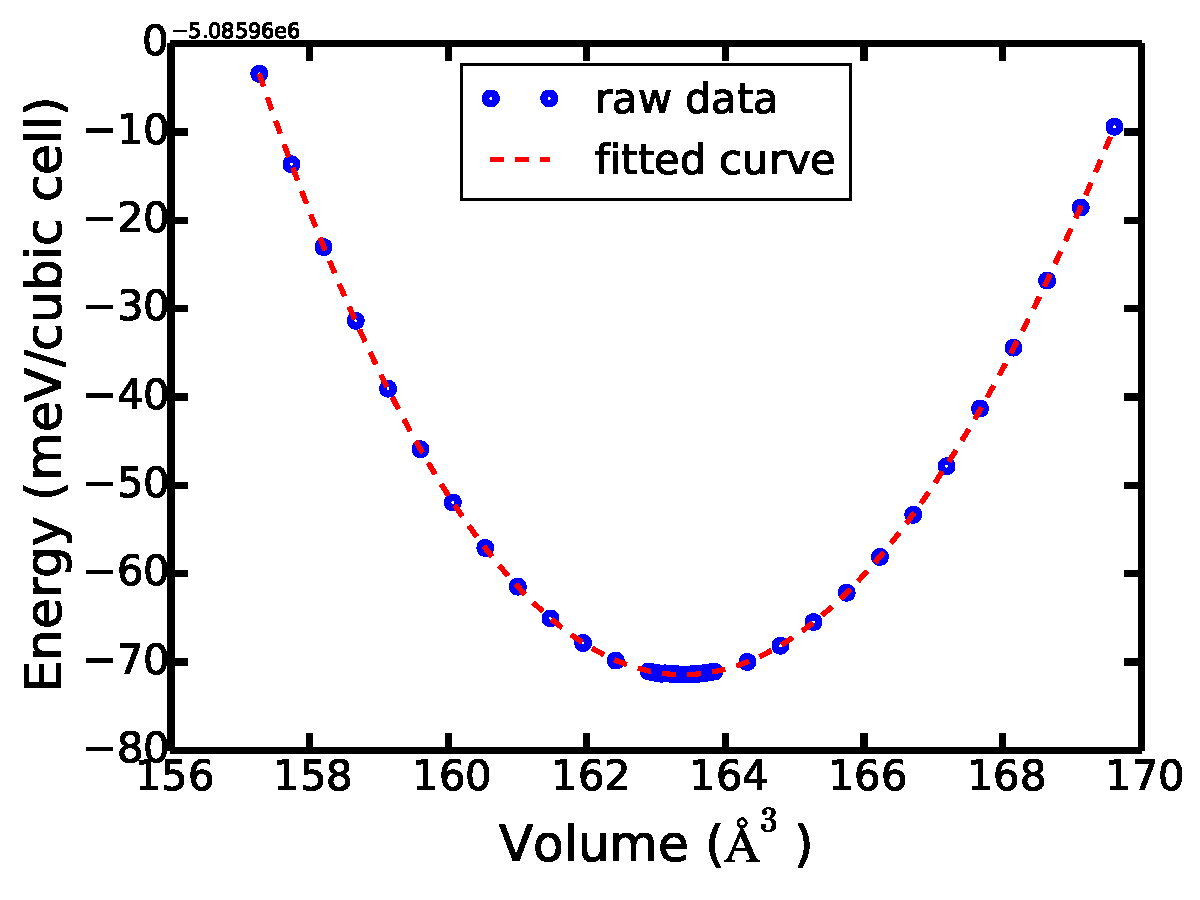
\includegraphics[width=.6\textwidth]{gga_v}
\end{center}
\end{figure}

The second derivative of energy at the equilibrium volume is calculated by fitting the curve to a 4-degree polynomial. 

\begin{flalign*}
K = V_0\left.\frac{\partial^2 E}{\partial V^2}\right|_{V = V_0} = 89.4 \unit{GPa}
\end{flalign*}

The calculated bulk modulus is slightly smaller than the experimental value of 97.6\unit{GPa}. 

\section*{Q9}

Except for using LDA, applied the same input parameters from previous section. Perform static calculations near the lattice constant at equilibrium. Plot the total energy (per cubic cell) as a function of lattice constant. 

\clearpage
\begin{figure}[h]
\begin{center}
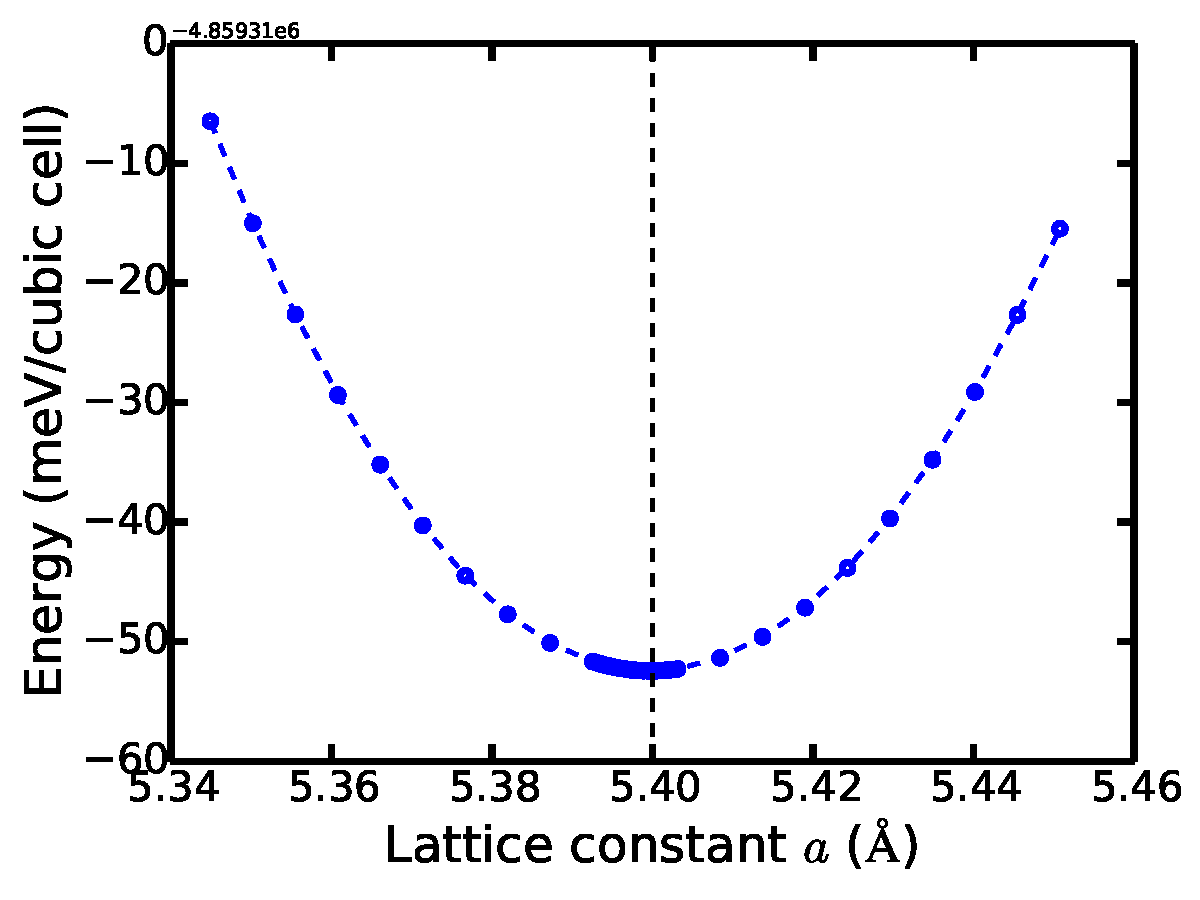
\includegraphics[width=.6\textwidth]{lda_a}
\end{center}
\end{figure}

The lattice constant of equilibrium structure is $a_0 = 10.204\unit{a.u.} = 5.4000\unit{\AA}$. This value is smaller than experimental one and the one obtained using GGA. 

Use the same procedure as in previous section to get the bulk modulus. 

\begin{figure}[h]
\begin{center}
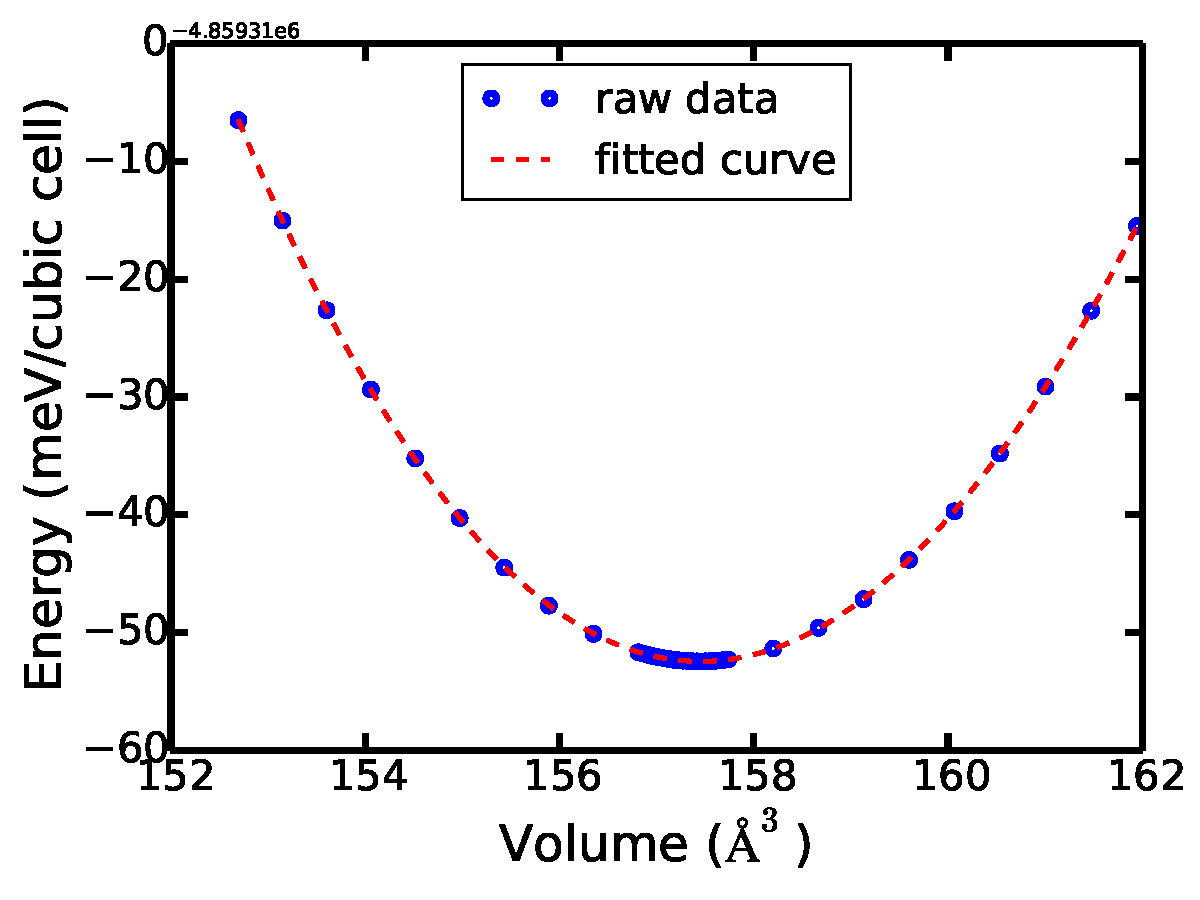
\includegraphics[width=.6\textwidth]{lda_v}
\end{center}
\end{figure}

\begin{flalign*}
K = V_0\left.\frac{\partial^2 E}{\partial V^2}\right|_{V = V_0} = 97.1 \unit{GPa}
\end{flalign*}

The calculated bulk modulus from LDA is surprisingly in good agreement with the experimental value of 97.6\unit{GPa}. 

\end{document}